% !TeX root = ../main.tex
\section{Уравнения, не разрешённые относительно производной}

В этом разделе $p=y'$. Система $F(x,y,p)=F_p(x,y,p)=0$ даёт
\emph{кандидатов} на особые решения. Каждый кандидат необходимо
подставить в исходное уравнение; одного обращения $F_p$ в нуль недостаточно.
Кроме отдельных гладких семейств, для уравнений первого порядка
ниже указаны возможные $C^1$-склейки с огибающими.

\task{Ф. 278}{Семейство парабол и его огибающая}
\sourcepage{33--35}
\[
 (y')^2-2xy'=x^2-4y.
\]
Выразим функцию через $x,p$:
\[
 y=\frac{x^2}4+\frac{xp}2-\frac{p^2}4.
\]
Дифференцируя и используя $\dd y=p\dd x$, получаем
\[
 (p-x)(\dd x+\dd p)=0.
\]
При $p=x$ находим $y=x^2/2$. На остальных гладких участках
$\dd p=-\dd x$, то есть $p=C-x$, и
\[
 y=-\frac{x^2}2+Cx-\frac{C^2}4.
\]
\answer{Обычное семейство:
$\displaystyle y=-\frac{x^2}2+Cx-\frac{C^2}4$.
Особое решение: $\displaystyle y=\frac{x^2}2$.}
Действительно, $F=p^2-2xp-x^2+4y$, $F_p=2p-2x$.
При $p=x$ система $F=F_p=0$ даёт $y=x^2/2$, и подстановка подтверждает
решение. Член семейства с $C=2a$ касается огибающей при $x=a$:
\[
 y_C=\frac{x^2}2-(x-a)^2,\qquad
 y_C(a)=\frac{a^2}2,\quad y'_C(a)=a.
\]
Все максимальные $C^1$-решения удобно записать так:
\[
 y(x)=\begin{cases}
 \frac{x^2}2-(x-a)^2,&x<a,\\
 \frac{x^2}2,&a\le x\le b,\\
 \frac{x^2}2-(x-b)^2,&x>b,
 \end{cases}
 \qquad -\infty\le a\le b\le+\infty.
\]
Бесконечный конец означает отсутствие соответствующей внешней ветви;
$a=b$ даёт одну обычную параболу, а оба бесконечных конца --- огибающую.
Для проверки полноты положим $w=x^2/2-y$. Исходное уравнение равносильно
$(w')^2=4w$, откуда $w\ge0$. На каждом положительном участке
$\sqrt w$ имеет постоянную производную $+1$ или $-1$;
между двумя нулями положительный участок невозможен. Это и даёт
указанную структуру.

\begin{center}
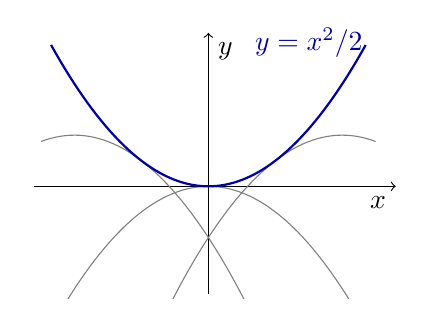
\begin{tikzpicture}[x=.85cm,y=.65cm]
 \clip (-2.7,-2.2) rectangle (2.9,3.1);
 \draw[->] (-2.6,0)--(2.8,0) node[below left] {$x$};
 \draw[->] (0,-2.1)--(0,3) node[below right] {$y$};
 \foreach \c in {-2,0,2}{
  \draw[gray,domain=-2.5:2.5,samples=70] plot(\x,{-.5*\x*\x+\c*\x-\c*\c/4});}
 \draw[thick,blue!65!black,domain=-2.35:2.35,samples=70] plot(\x,{.5*\x*\x});
 \node[blue!65!black] at (1.5,2.8) {$y=x^2/2$};
\end{tikzpicture}
\end{center}

\task{Ф. 287}{Уравнение Клеро}
\sourcepage{35--36}
\[
 y=xy'-(y')^2.
\]
С $p=y'$ имеем $y=xp-p^2$ и
\[
 p\dd x=p\dd x+(x-2p)\dd p,
 \qquad (x-2p)\dd p=0.
\]
При $p=C$ получаем прямые $y=Cx-C^2$; при $p=x/2$ --- параболу $y=x^2/4$.
\answer{$y=Cx-C^2$ и особое решение $y=x^2/4$.}
Система $F=y-xp+p^2=0$, $F_p=-x+2p=0$ даёт ту же параболу.
Прямая с $C=a/2$ касается её в точке $(a,a^2/4)$.
Все максимальные $C^1$-решения, включая склейки, имеют вид
\[
 y(x)=\begin{cases}
 \frac a2x-\frac{a^2}4,&x<a,\\
 \frac{x^2}4,&a\le x\le b,\\
 \frac b2x-\frac{b^2}4,&x>b,
 \end{cases}\qquad -\infty\le a\le b\le+\infty.
\]
Как и выше, бесконечные концы допускаются. Чтобы увидеть полноту,
положим $w=x^2/4-y$. Тогда $w=(p-x/2)^2=(w')^2$;
на положительных участках $(\sqrt w)'=\pm1/2$.
\begin{center}
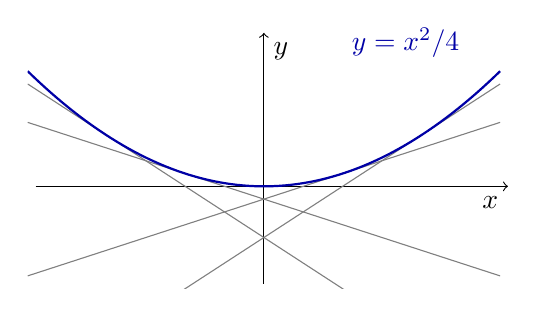
\begin{tikzpicture}[x=1cm,y=.65cm]
 \clip (-3,-2) rectangle (3.2,3.1);
 \draw[->] (-2.9,0)--(3.1,0) node[below left] {$x$};
 \draw[->] (0,-1.9)--(0,3) node[below right] {$y$};
 \foreach \c in {-1,-.5,.5,1}{
  \draw[gray,domain=-3:3,samples=2] plot(\x,{\c*\x-\c*\c});}
 \draw[thick,blue!65!black,domain=-3:3,samples=80] plot(\x,{\x*\x/4});
 \node[blue!65!black] at (1.8,2.8) {$y=x^2/4$};
\end{tikzpicture}
\end{center}

\task{Ф. 288}{Параметрическое решение}
\sourcepage{36--37}
\[
 y+xy'=4\sqrt{y'},\qquad p=y'\ge0.
\]
Случай $p\equiv0$ даёт $y\equiv0$. При $p>0$ имеем
$y=4\sqrt p-xp$. Дифференцируем:
\[
 2p\dd x+\left(x-\frac2{\sqrt p}\right)\dd p=0.
\]
Считая $x=x(p)$, получаем линейное уравнение
\[
 \frac{\dd x}{\dd p}+\frac{x}{2p}=p^{-3/2},\qquad
 \frac{\dd}{\dd p}(x\sqrt p)=\frac1p.
\]
Отсюда
\answer{$\displaystyle
 x(p)=\frac{\ln p+C}{\sqrt p},\qquad
 y(p)=\sqrt p\,(4-\ln p-C),\qquad p>0$,
а также $y\equiv0$.}
В обеих координатах используется \emph{одна и та же} константа.
В рукописи перед $C\sqrt p$ во второй координате ошибочно стоит плюс.
Непосредственная проверка исправленной формулы:
\[
 y+xp=\sqrt p(4-\ln p-C)+\sqrt p(\ln p+C)=4\sqrt p.
\]
Кроме того,
\[
 x_p=\frac{2-\ln p-C}{2p^{3/2}},\qquad y_p=p\,x_p.
\]
На участках $x_p\ne0$ это доказывает $\dd y/\dd x=p$.
Точка $p=e^{2-C}$ разделяет параметрическую кривую на две ветви графика.
Кандидат из $F_p=x-2/\sqrt p=0$ даёт $y=4/x$, $x>0$,
но у него $y'=-4/x^2<0$. Следовательно, он не является решением.
Нулевое решение нельзя потерять из-за деления на $p$.

\task{С. 6:7}{Две особые параболы}
\sourcepage{38--39}
\[
 (y')^3-3x^2y'+4xy=0.
\]
При $x\ne0$ выражаем $y$ через $p$:
\[
 y=\frac34xp-\frac{p^3}{4x}.
\]
Дифференцирование с учётом $\dd y=p\dd x$ даёт
\[
 \left(1-\frac{p^2}{x^2}\right)(p\dd x-3x\dd p)=0.
\]
Первый множитель даёт $p=\pm x$ и $y=\pm x^2/2$.
Из второго получаем $p=A\sqrt[3]x$, включая $A=0$, и
\[
 y=\frac{3A}4x^{4/3}-\frac{A^3}4.
\]
Переобозначая $A=4C$, записываем
\answer{$\displaystyle y=3Cx^{4/3}-16C^3$, $C\in\R$;
особые решения $\displaystyle y=\pm\frac{x^2}2$.}
Эти формулы имеют непрерывную первую производную и при $x=0$.
Там исходное уравнение требует лишь $y'(0)=0$, что выполнено.

Для поиска особых решений $F_p=3p^2-3x^2=0$ даёт $p=\pm x$;
обе соответствующие параболы удовлетворяют исходному уравнению.
При касании верхней параболы в точке $a\ne0$:
\[
 4C\sqrt[3]a=a,\qquad C=\frac{|a|^{2/3}}4,
\]
а нижней --- $C=-|a|^{2/3}/4$. Подстановка в семейство даёт
соответственно $\pm a^2/2$ и тот же наклон $\pm a$.
В нуле обе параболы касаются решения $y=0$.

Возможны также $C^1$-склейки указанных ветвей в точках касания.
Например, при $C>0$ один член семейства касается верхней параболы
в двух точках $a=\pm(4C)^{3/2}$; между точками можно выбрать этот
член семейства, а вне них --- верхнюю параболу.
Для $C<0$ аналогично используется нижняя парабола.
При переходе через нуль верхняя и нижняя параболы также могут
склеиваться друг с другом или с $y=0$.

\begin{center}
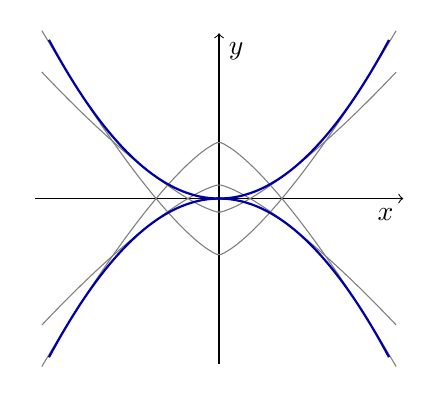
\begin{tikzpicture}[x=.9cm,y=.7cm]
 \clip (-2.7,-3.1) rectangle (2.7,3.1);
 \draw[->] (-2.6,0)--(2.6,0) node[below left] {$x$};
 \draw[->] (0,-3)--(0,3) node[below right] {$y$};
 \foreach \c in {-.4,-.25,.25,.4}{
  \draw[gray,domain=-2.5:2.5,samples=100] plot(\x,{3*\c*pow(abs(\x),1.333333)-16*\c*\c*\c});}
 \draw[thick,blue!65!black,domain=-2.4:2.4,samples=80] plot(\x,{.5*\x*\x});
 \draw[thick,blue!65!black,domain=-2.4:2.4,samples=80] plot(\x,{-.5*\x*\x});
\end{tikzpicture}
\end{center}

\task{Д. 5, а, б}{Два условия и склейки с огибающей}
\sourcepage{40}
На этой странице уравнение не выписано, но использованы прямые
$y=Cx-C^2$ и парабола $y=x^2/4$. Следовательно, решение относится к
уравнению Клеро из Ф.\,287:
\[
 y=xy'-(y')^2.
\]
Ниже восстановлены условия именно для этого уравнения.

\textbf{а)} $y(0)=-1$, $y(5)=6$.
Из $-C^2=-1$ следует $C=\pm1$.
Прямая $y=-x-1$ касается параболы при $x=-2$, то есть левее начальной
точки, и вправо от $0$ не может перейти на огибающую. Она не подходит.
Остаётся $y=x-1$ до точки касания $x=2$.

Чтобы достичь $(5,6)$, нужно сойти с огибающей на касательную
$y=Cx-C^2$. Условие $5C-C^2=6$ даёт $C=2$ или $C=3$.
Точки касания имеют абсциссы $2C=4$ и $2C=6$ соответственно.
Второй вариант не годится: при $x=5$ решение ещё лежало бы на
огибающей и имело значение $25/4\ne6$.
\answer{Единственное максимальное $C^1$-решение:
\[
 y(x)=\begin{cases}
 x-1,&x<2,\\
 x^2/4,&2\le x\le4,\\
 2x-4,&x>4.
 \end{cases}
\]}

\textbf{б)} $y(0)=-1$, $y(4)=4$.
До $x=2$ рассуждение то же. Точка $(4,4)$ лежит на огибающей.
Отойти от неё можно в любой момент $b\ge4$ или не отходить вовсе.
\answer{Все максимальные решения имеют вид
\[
 y_b(x)=\begin{cases}
 x-1,&x<2,\\
 x^2/4,&2\le x\le b,\\
 \frac b2x-\frac{b^2}4,&x>b,
 \end{cases}\qquad 4\le b\le+\infty.
\]
При $b=+\infty$ последняя ветвь отсутствует.}
На отрезке $[0,4]$ все решения совпадают; различаются их продолжения
вправо. В рукописи приведён только частный случай $b=4$.

\begin{center}
\begin{tikzpicture}[x=.8cm,y=.5cm]
 \draw[->] (-.5,0)--(6.3,0) node[right] {$x$};
 \draw[->] (0,-1.6)--(0,8.5) node[above] {$y$};
 \draw[dashed,gray,domain=0:5.7,samples=70] plot(\x,{\x*\x/4});
 \draw[thick,blue!65!black,domain=-.3:2] plot(\x,{\x-1});
 \draw[thick,blue!65!black,domain=2:4,samples=40] plot(\x,{\x*\x/4});
 \draw[thick,blue!65!black,domain=4:6] plot(\x,{2*\x-4});
 \fill (0,-1) circle(2pt) node[left] {$-1$};
 \fill (4,4) circle(2pt) node[below right] {$(4,4)$};
 \fill (5,6) circle(2pt) node[below right] {$(5,6)$};
 \node[below] at (2,0) {$2$};
\end{tikzpicture}
\end{center}
\editnote{В приложенной программе другого года похожая задача отсылает
к Ф.\,278, однако на странице 40 рукописи явно решается Ф.\,287.
Эта неоднозначность не скрыта заменой уравнения: здесь сохранено
содержание набираемой рукописи.}

\task{Д. 6}{Особое решение и задержка на нём}
\sourcepage{41--42}
\[
 (y')^2=4y^3(1-y).
\]
Правая часть неотрицательна только при $0\le y\le1$.
Постоянные $y=0$ и $y=1$ сразу проверяются.
Для $y>0$ положим $u=1/y$; тогда
\[
 (u')^2=4(u-1),\qquad u\ge1.
\]
При $u>1$ имеем $u'=\pm2\sqrt{u-1}$, откуда
$u=1+(x-C)^2$ на соответствующих ветвях.
\answer{Обычное семейство: $\displaystyle y=\frac1{1+(x-C)^2}$.
Отдельные постоянные решения: $y=0$ и $y=1$.}
Записи с $(x+C)^2$ и $(x-C)^2$ задают одно семейство при $C\in\R$,
поэтому дважды перечислять их не нужно.

Для $F=p^2-4y^3(1-y)$ равенство $F_p=2p=0$ даёт кандидатов $y=0,1$.
Семейство касается $y=1$ при $x=C$, с нулевой производной.
Поэтому $y=1$ --- особое решение, огибающая семейства.
Ни один его член не достигает $y=0$ при конечном $x$, поэтому
$y=0$ не является особым решением в этом смысле.

Полный список максимальных положительных $C^1$-решений включает
произвольное время пребывания на уровне $1$:
\[
 y(x)=\begin{cases}
 \dfrac1{1+(x-a)^2},&x<a,\\[2pt]
 1,&a\le x\le b,\\[2pt]
 \dfrac1{1+(x-b)^2},&x>b,
 \end{cases}\qquad -\infty\le a\le b\le+\infty.
\]
Дополнительно имеется $y\equiv0$. При $a=b$ получаем обычный член
семейства, при бесконечных концах --- решения с одной внешней ветвью
или $y\equiv1$. В местах склейки производная равна нулю.
Полнота следует из того, что $v=u-1$ удовлетворяет $(v')^2=4v$;
между двумя нулями оно не может иметь положительного участка.

От уровня $0$ нельзя отойти за конечное время: при $0\le y\le1$
выполнено $|y'|=2y^{3/2}\sqrt{1-y}\le2y$.
Если $y(x_0)=0$, интегральное неравенство и лемма Гронуолла
(в обе стороны от $x_0$) дают $y\equiv0$. Поэтому в отличие от
уровня $1$ задержки на уровне $0$ новых решений не создают.

\begin{center}
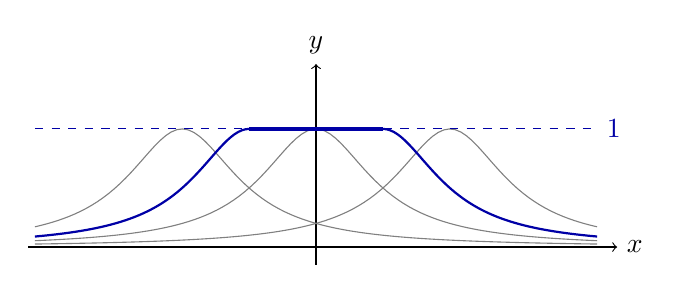
\begin{tikzpicture}[x=.85cm,y=1.5cm]
 \draw[->] (-4.3,0)--(4.5,0) node[right] {$x$};
 \draw[->] (0,-.15)--(0,1.55) node[above] {$y$};
 \foreach \c in {-2,0,2}{
  \draw[gray,domain=-4.2:4.2,samples=100] plot(\x,{1/(1+(\x-\c)^2)});}
 \draw[dashed,blue!65!black] (-4.2,1)--(4.2,1) node[right] {$1$};
 \draw[thick,blue!65!black,domain=-4.2:-1,samples=60] plot(\x,{1/(1+(\x+1)^2)});
 \draw[very thick,blue!65!black] (-1,1)--(1,1);
 \draw[thick,blue!65!black,domain=1:4.2,samples=60] plot(\x,{1/(1+(\x-1)^2)});
\end{tikzpicture}
\end{center}
